
\chapter{Text Mining}

\section{Text Mining in General}

There is a fast growing amount of \emph{structured data} in the form of very large databases, numerical data collections, multimedia data and log files, commonly referred to as \emph{Big Data} nowadays.
\emph{Data mining} -- also known as \emph{knowledge discovery} from data -- is about the discovery of interesting patterns in huge data collections through computational analysis \citep{han2006data}.
In addition, however, there is a parallel stream of so-called \emph{unstructured data} in the form of text.
This comprises traditional text sources such as newspapers, books, magazines and journals, as well as new media such webpages (Wikipedia, IMDB), blogs, social media (Facebook) and messaging (Twitter,SMS).
Much of the collective knowledge of the human race has historically been encoded in the form of text. 
Data mining methods can not handle text as input.
Therefore text needs to be converted to some form of structured data first in order to apply data mining techniques.
This is essentialy what \emph{text mining} is about: extracting structured information from text in order to discover patterns in huge text collections through automated processing.

Text mining is applied in many different areas and for many different purposes; for a recent overview see e.g. \citep{Aggarwal2012Mining,Weiss2012Fundamentals}.
Different domains require different approaches, techniques, tools and resources.
For example, opinion mining regarding movies from social media is quite different from trend detection in financial markets. 
In this report we focus on text mining of scientfic literature to support knowledge discovery, of which literature-based discovery is a particular variant.
Mining of scientific literature is commonly regarded as a combination of four tasks: information retrieval, information extraction, natural language processing and data mining.

\emph{Information retrieval} (IR) addresses the task of searching a large document collection for documents that are relevent to a user's informational needs as expressed in a search query \citep{ManningRaghavanSchutze:08}. 
The most common IR applications nowadays are web search engines which try to retrieve relevant text documents from the web, mostly webpages, given a number of keywords or phrases.
Specialized search engines exists for particular documents collections, for instance, to search scientific publications in the area of biomedicine (PUBMED), because additional knowledge about the domain can be used to improve IR results.
IR is typically the first step in text mining in order to narrow down the set of relevant documents to a size managable for more in depth analysis.

\emph{Information extraction} (IE) is the process of automatically extracting structured information from text \citep{Jiang2012Information}.
What type of structured information is extracted depends on the application, but usually involves two general types of information: \emph{entities} and \emph{relations}.
Entities are the things mentioned in the text.
These can be general categories like people, organisations, companies or places, but can also be domain-specific such as proteins, genes, drugs, organisms or anatomical parts.
Finding entities in text is called \emph{named entity recognition} or \emph{entity detection}.
Relations hold among pairs of entities.
For example, a company can \emph{buy} another company, a certain protein may \emph{interact} with a certain gene, or a certain drug may \emph{cause} a certain side effect.
The task of finding predefined relations in text is known as \emph{relation extraction}.  
Relations may be more complex than simple binary relations between pairs of entities.
They may involve multiple entities playing different roles, with additional circumstances or conditions, or even relations between relations.
In this case, it is common to talk about \emph{events} and the task of \emph{event extraction}.

\emph{Natural language processing} (NLP) concerns automatic analysis of language by computers, usually from an applied point of view  \citep{jurafsky2000speech,manning1999foundations}.
Natural languages such as English or Chinese -- as opposed to artificial languages like traffic signs or programming languages -- are extremely complex and versatile symbolic systems that have evolved over time to enable humans to exchange information.
Language can convey many different types of information, ranging from simple facts to complex arguments or emotional states.
Notwithstanding tremendous progress in NLP over the last decades, computers are still far from really understanding language and currently manage a shallow grasp of meaning at best.
In practice, NLP for a specific domain, e.g. stock market reports or biomedical research articles, works significantly better than NLP for unrestricted input, because domain-specific language use and knowledge can be exploited to improve interpretation. 
Hence NLP techniques, tools and resources are often tied to a particular application domain.

Most IR systems rely to some extent on NLP.
Key word search, for instance, often involves a \emph{lemmatisation} step wich relates all morphological variants of a word to its stem.
For example, the verbs \emph{diving}, \emph{dives}, \emph{dove}, \emph{dived} are all linked to their base form \emph{dive}.
For many languages, this improves the recall of relevant documents at the (slight) expense of precision, i.e., some extra irrelevant documents are returned.
More advanced NLP techniques are keyword expansion with automatically learned synonymns and word sense disambiguation for keywords with more than one possible interpretation.  

IE tends to be highly dependent on NLP for linguistic analysis and interpretation of the input text prior to actual extraction.
Common NLP techniques are \emph{part-of-speech tagging} (labeling tokens according to their word class, such a noun, verb, preposition, etc.), lemmatisation (bringing back words to their lemma form) and syntactic parsing (analysis of the grammatical structure of sentences).
The resulting linguistic annotations of the text serve as input to the algorithms for entity recognition and relation extraction, which can range from hand-written pattern matching rules to data-driven machine learning algorithms that learn from examples..
Like domain-specific NLP, IE is usually rather restricted in scope.
That is, it targets a small subset of specific entities and relations of interest in the given domain, ignoring all other meaning contained in the text.    

Even with these limitations to a particular domain and to particular aspects of meaning, computers still make many mistakes in processing text, misinterpreting text and failing to detect important information.
Despite all their limitations, computers have one major advantage over humans when it comes to reading text: processing power.
Computers can process thousands or millions of documents in a relatively short time, something a human reader would never be able to match.
The main strenght of text mining thus comes from the ability to process big text data.
One of the challenges is how best to combine the fast but shallow and noisy processing capabilities of text mining systems with the slow but deep language understanding capibilities of humans.
This relates to the fields of human-computer interaction and information visualisation.   

\section{Text Mining Applications in Biomedicine}
\label{sec:tm-biomed}

The first and most active area for research on, and application of, text mining is that of scientific publications in the fields of biology and medicine, collectively referred to as \emph{biomedicine}.
One of the main reasons for this is the volume and rate of publications in biomedicine.
The MEDLINE (Medical Literature Analysis and Retrieval System Online) is a bibliographic database which indexes most biomedical publications from over 5,5000 journals since the 1950s.
Abstracts are searchable with PubMed, which currently contains over 23 million records and grows at a rate of approximately three publications a minute.
Full-text articles can be searched with PubMed Central and many alternative or specialized search engines are available. 
Even though these allow researchers to retrieve documents by means of keyword search, and refine search results in different ways, search queries may still return thousands of hits and checking all of them for relevant information is practically infeasible.
Text mining tools can offer a solution.
They can be be used for tasks such as further filtering of documents, clustering similar documents, automatically extracting information of interest, summarizing information through text and/or visualisation, and discovering regularities or inconsistencies.

There are already many excellent survey and review articles about text mining in biomedicine, including
\citep{Neves2012Survey,Simpson2012Biomedical,Andronis2011Literature,Ananiadou2010Event,RodriguezEsteban2009Biomedical,Zweigenbaum2009Advanced,Cohen2008Getting,Zweigenbaum2007Frontiers,Ananiadou2006,Erhardt2006Status,JenEA06,Spasic2005Text,Cohen2005Survey,Krauthammer2004Term,Blake2011Text,Krallinger2010Analysis}.
Since we do not want to duplicate these efforts with yet another survey, our discussion here is limited to a couple of examples of text mining applications in biology and medicine.

The Information Hyperlinked Over Proteins\footnote{\url{http://www.ihop-net.org}} (iHop) system \citep{hoffmann2004gene} is a free online service that provides access to hyperlinked versions of abstracts from PubMed, a large database containing millions of abstract from journal articles in biomedicine.
Every occurrence of an enitity, such as a gene or a protein, is hyperlinked to its occurrences in other abstracts, making it easy to hop from one sentence/abstract to another one.
Given a gene, users can search for other genes that it interacts with (Figure~\ref{fig:ihop-1}), go on to a list of sentences where the interactions are extracted from (Figure~\ref{fig:ihop-2}) , and go on from sentences to the abstracts they originate from  (Figure~\ref{fig:ihop-3}).   
Interactions can be stored to build an interaction graph where nodes are genes and edges are links to sentences entailing the interaction. 

\begin{figure}
\begin{center}
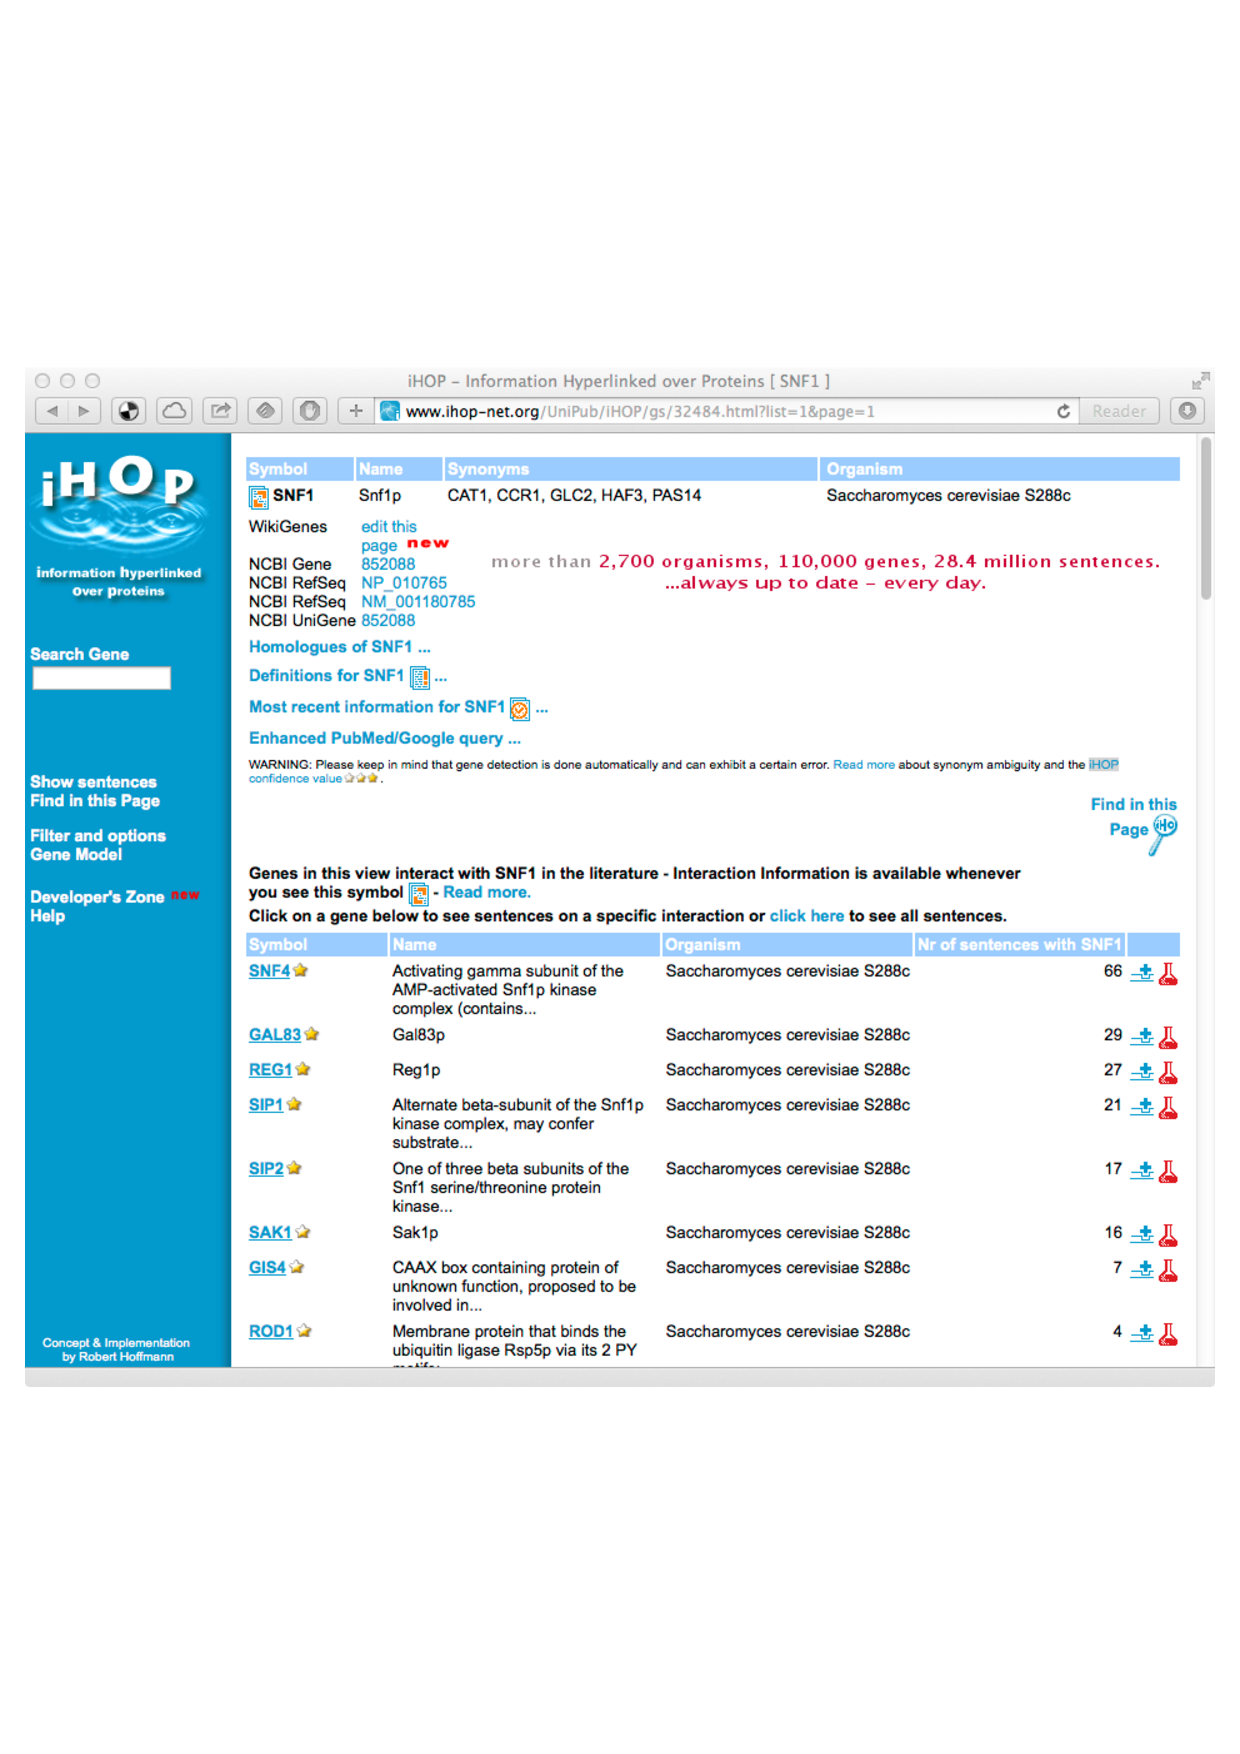
\includegraphics[scale=0.6]{figures/ihop-1.pdf}
 \caption{iHop view of interacting genes }
\label{fig:ihop-1}
\end{center}
\end{figure}    

\begin{figure}
\begin{center}
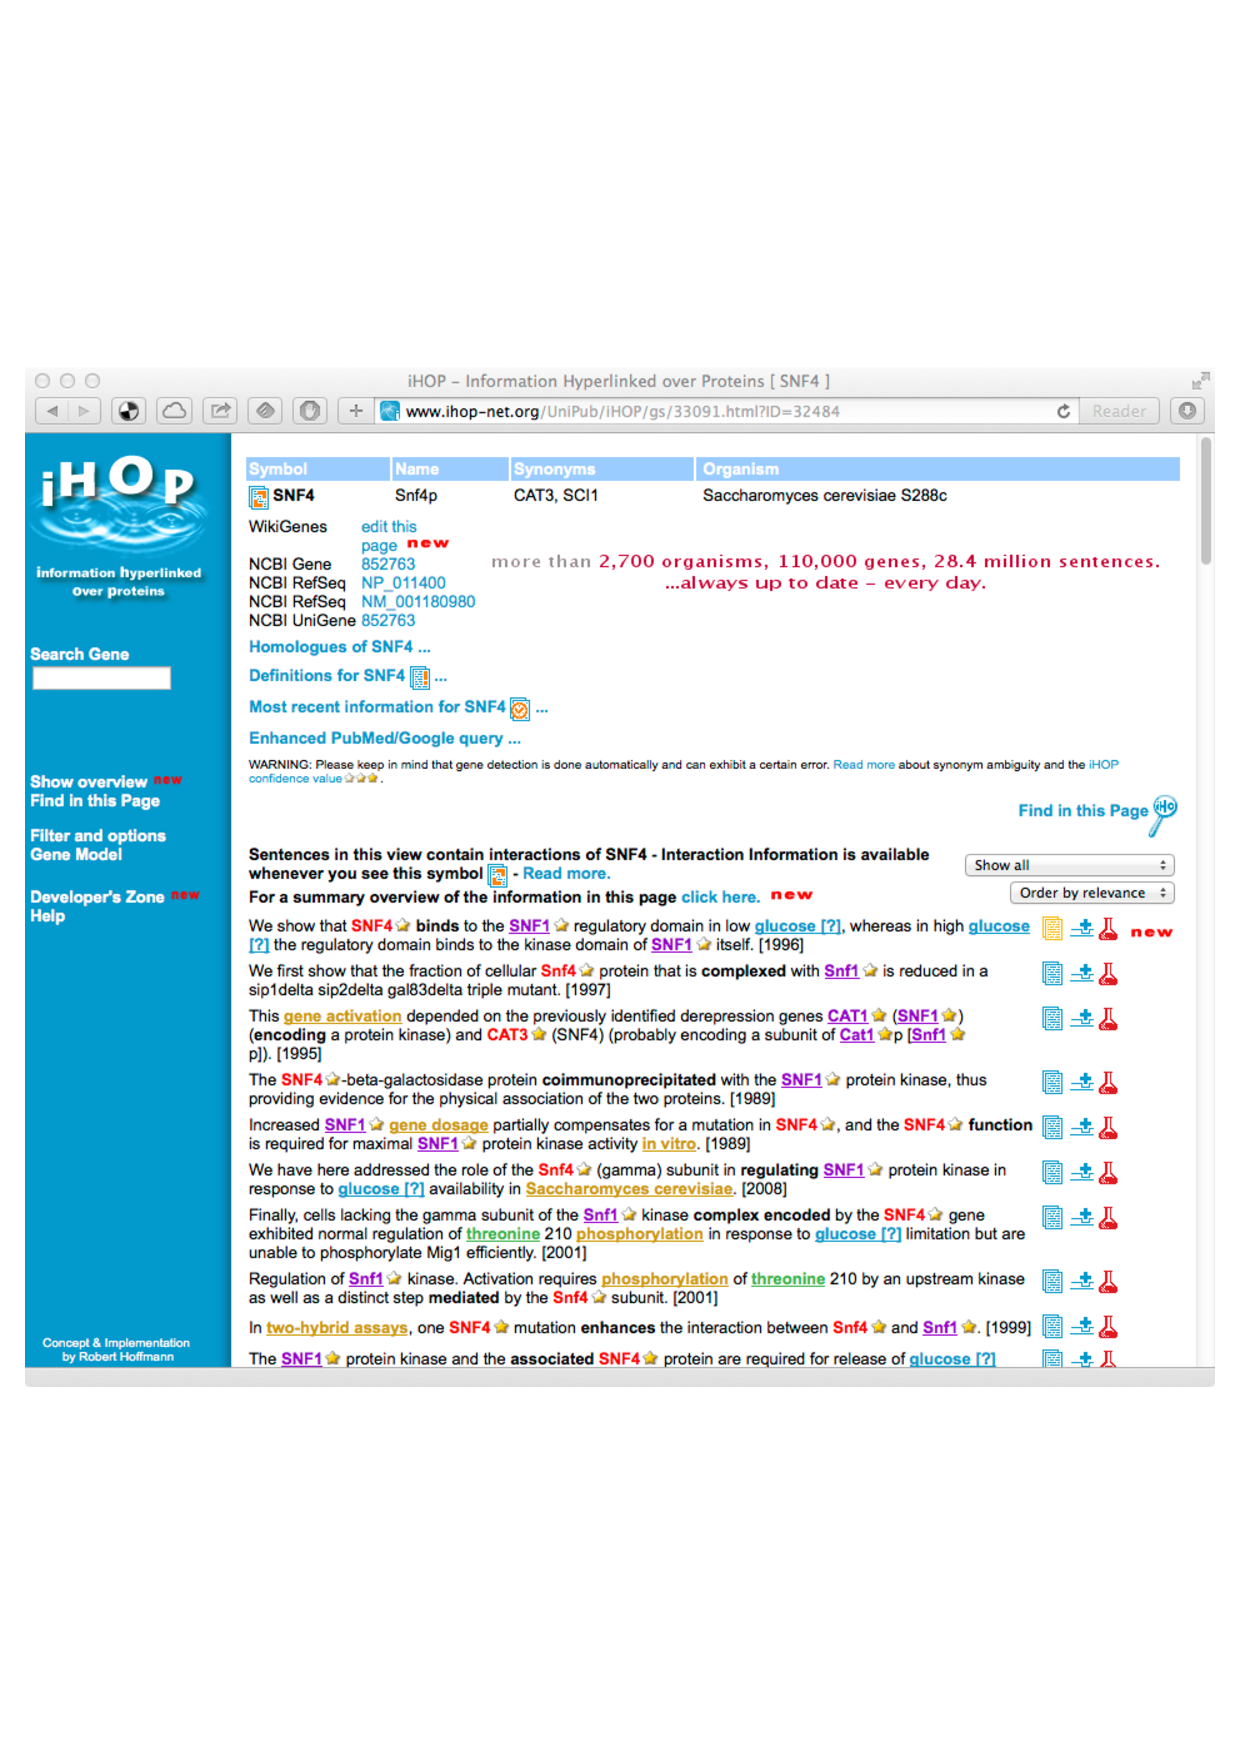
\includegraphics[scale=0.6]{figures/ihop-2.pdf}
 \caption{iHop view of sentences describing interactions}
\label{fig:ihop-2}
\end{center}
\end{figure}

\begin{figure}
\begin{center}
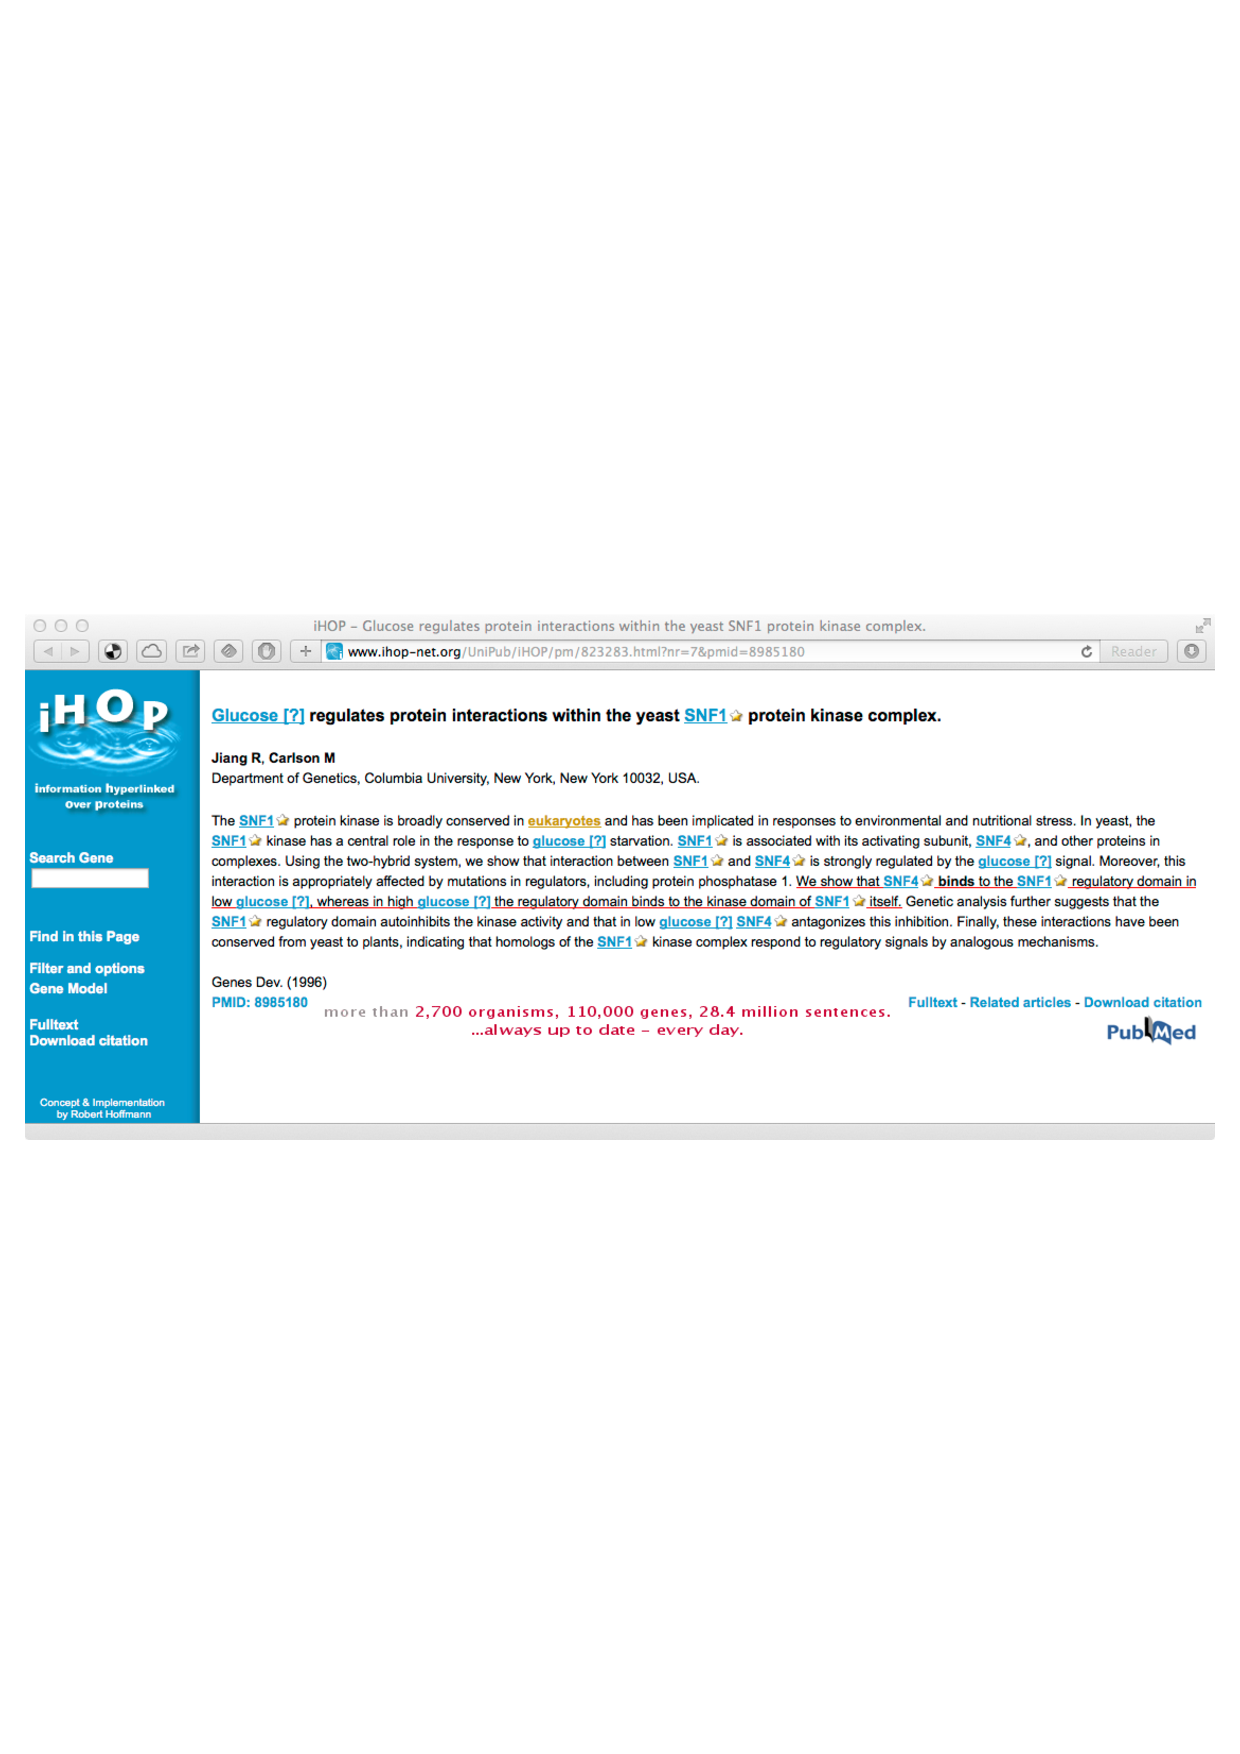
\includegraphics[scale=0.6]{figures/ihop-3.pdf}
 \caption{iHop view of hyperlinked abstract}
\label{fig:ihop-3}
\end{center}
\end{figure}

Chilibot\footnote{\url{http://www.chilibot.net}} is a similar webservice for searching PubMed abstracts \citep{Chen2004Contentrich}.
Users can search for interactions between a pairs of genes or proteins.
List of terms can be supplied to perform exhaustive searches of all possible relationships between any two terms in a list.
Search results can be further constrainted by any number of free-text keywords.
In addition, there are special keywords like \emph{modulate} that triggers a search for regulatory relationships (inhibition, stimulation, increase, reduce, etc.),  
The system returns sentences describing these interactions, linked to the abstacts they originate from.
The results are also presented as a summary graph, with nodes representing the queried terms and edges representing the relationships.

FACTA+\footnote{\url{http://www.nactem.ac.uk/facta/}} is a webservice for discovering associations between biomedical entities: gene/protein, disease, symptom, drug, enzyme, compound \citep{Tsuruoka2008FACTA}.
It indexes all abstracts in MedLine and allows users to navigate the associations and the textual evidence in an intuitive way.
Figure~\ref{fig:facta} shows FACTA+ presenting concepts associated to ``caffeine''.
Associated concepts are organized per entity class and ranked according to their association strength.
Several different measures are supported, e.g. frequency and mutual information.
Clicking on the document icon present a list of text snippets that are the source for the associations, including a link to the full abstract.
Clicking on any concept results in a new search for concepts associated to that concepts. 

In addition, it is possibly to search for indirectly related concepts through a \emph{pivot} concept.
This is akin to the ABC-linking in literature-based discovery.
Both pivot concepts and target concepts can be restricted to a certain type, for example, protein and disease.

The service has recetly been extended with a graphical visualisation component\footnote{\url{http://www.nactem.ac.uk/facta-visualizer/}}.
Figure~\ref{fig:facta-vis} shows 
This interactive visualisation also allows following links to text evidence and visualising indirect associations.

\begin{figure}
\begin{center}
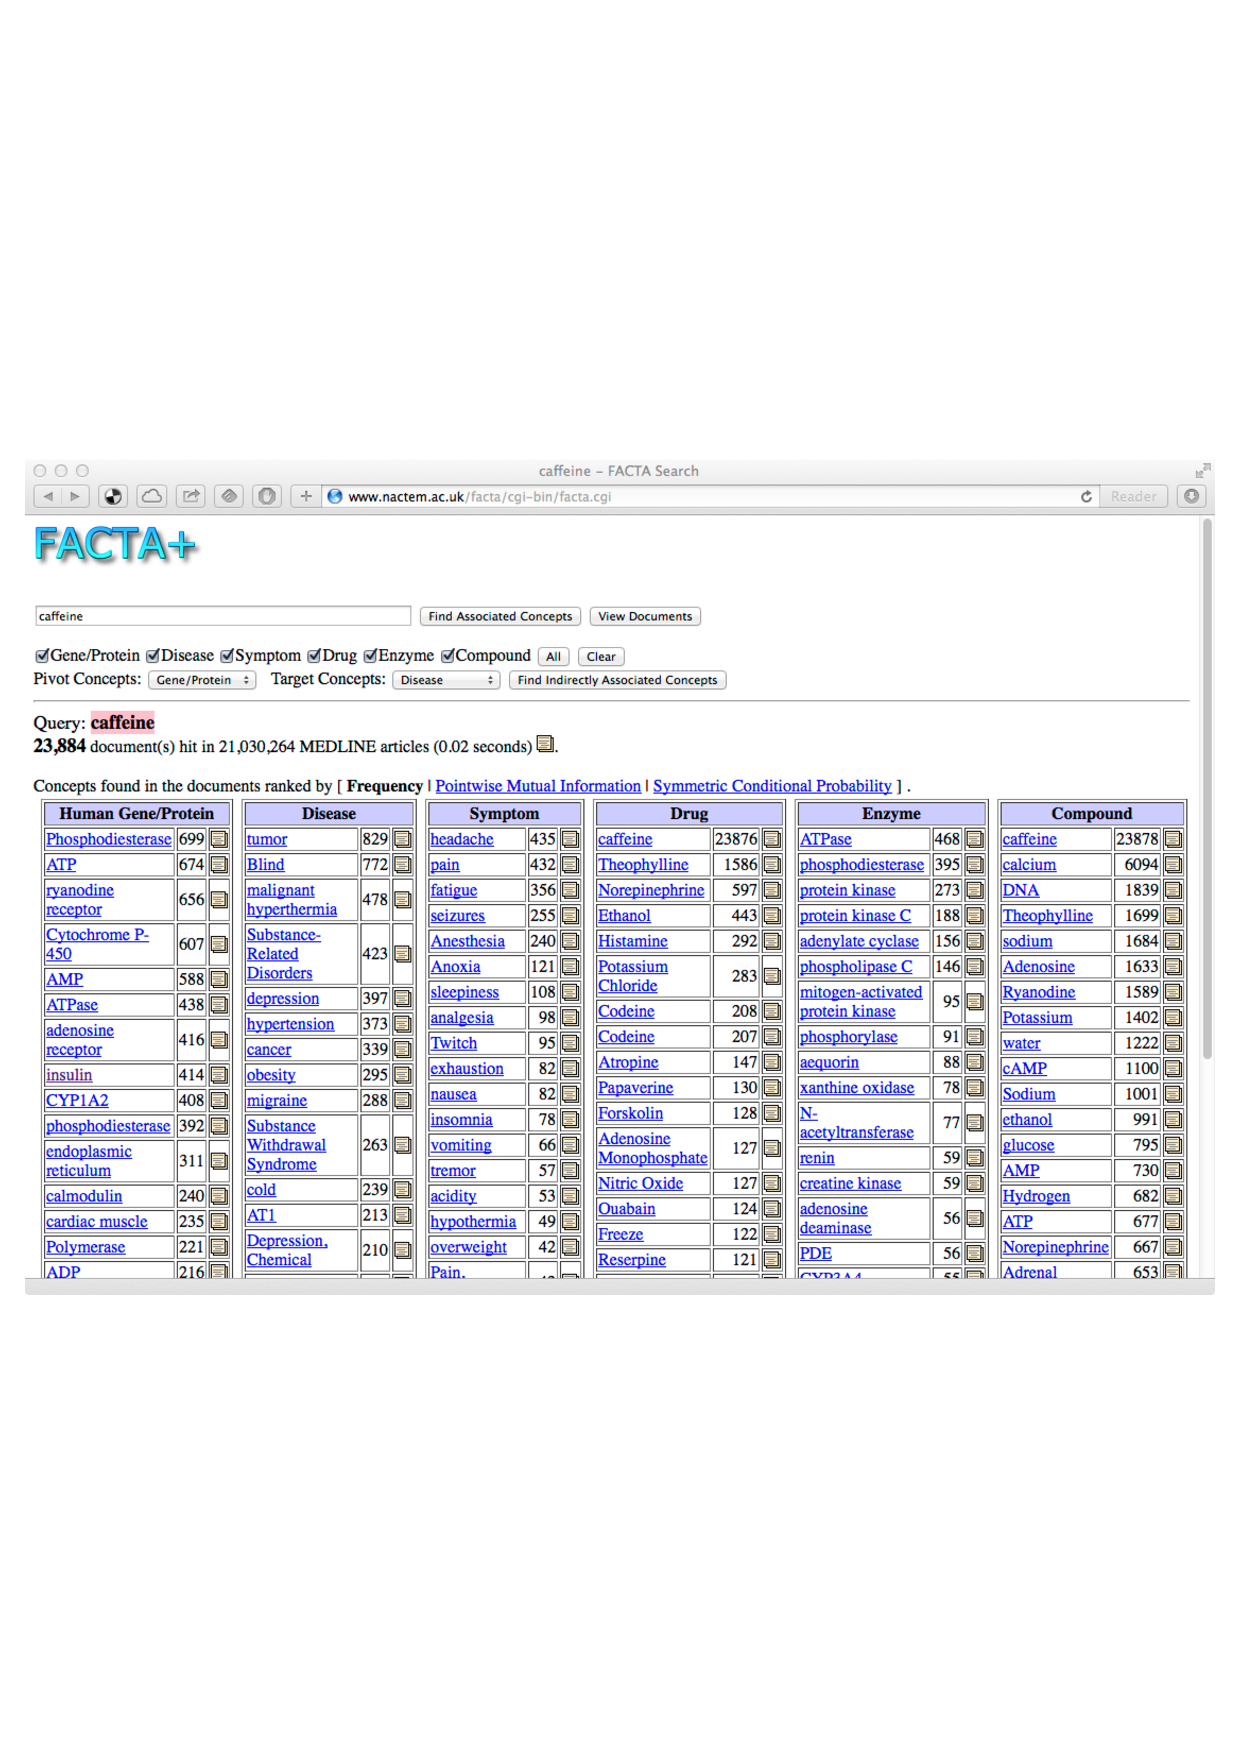
\includegraphics[scale=0.6]{figures/facta.pdf}
 \caption{FACTA+ showing concepts associated to ``caffeine'' }
\label{fig:facta}
\end{center}
\end{figure}
  
\begin{figure}
\begin{center}
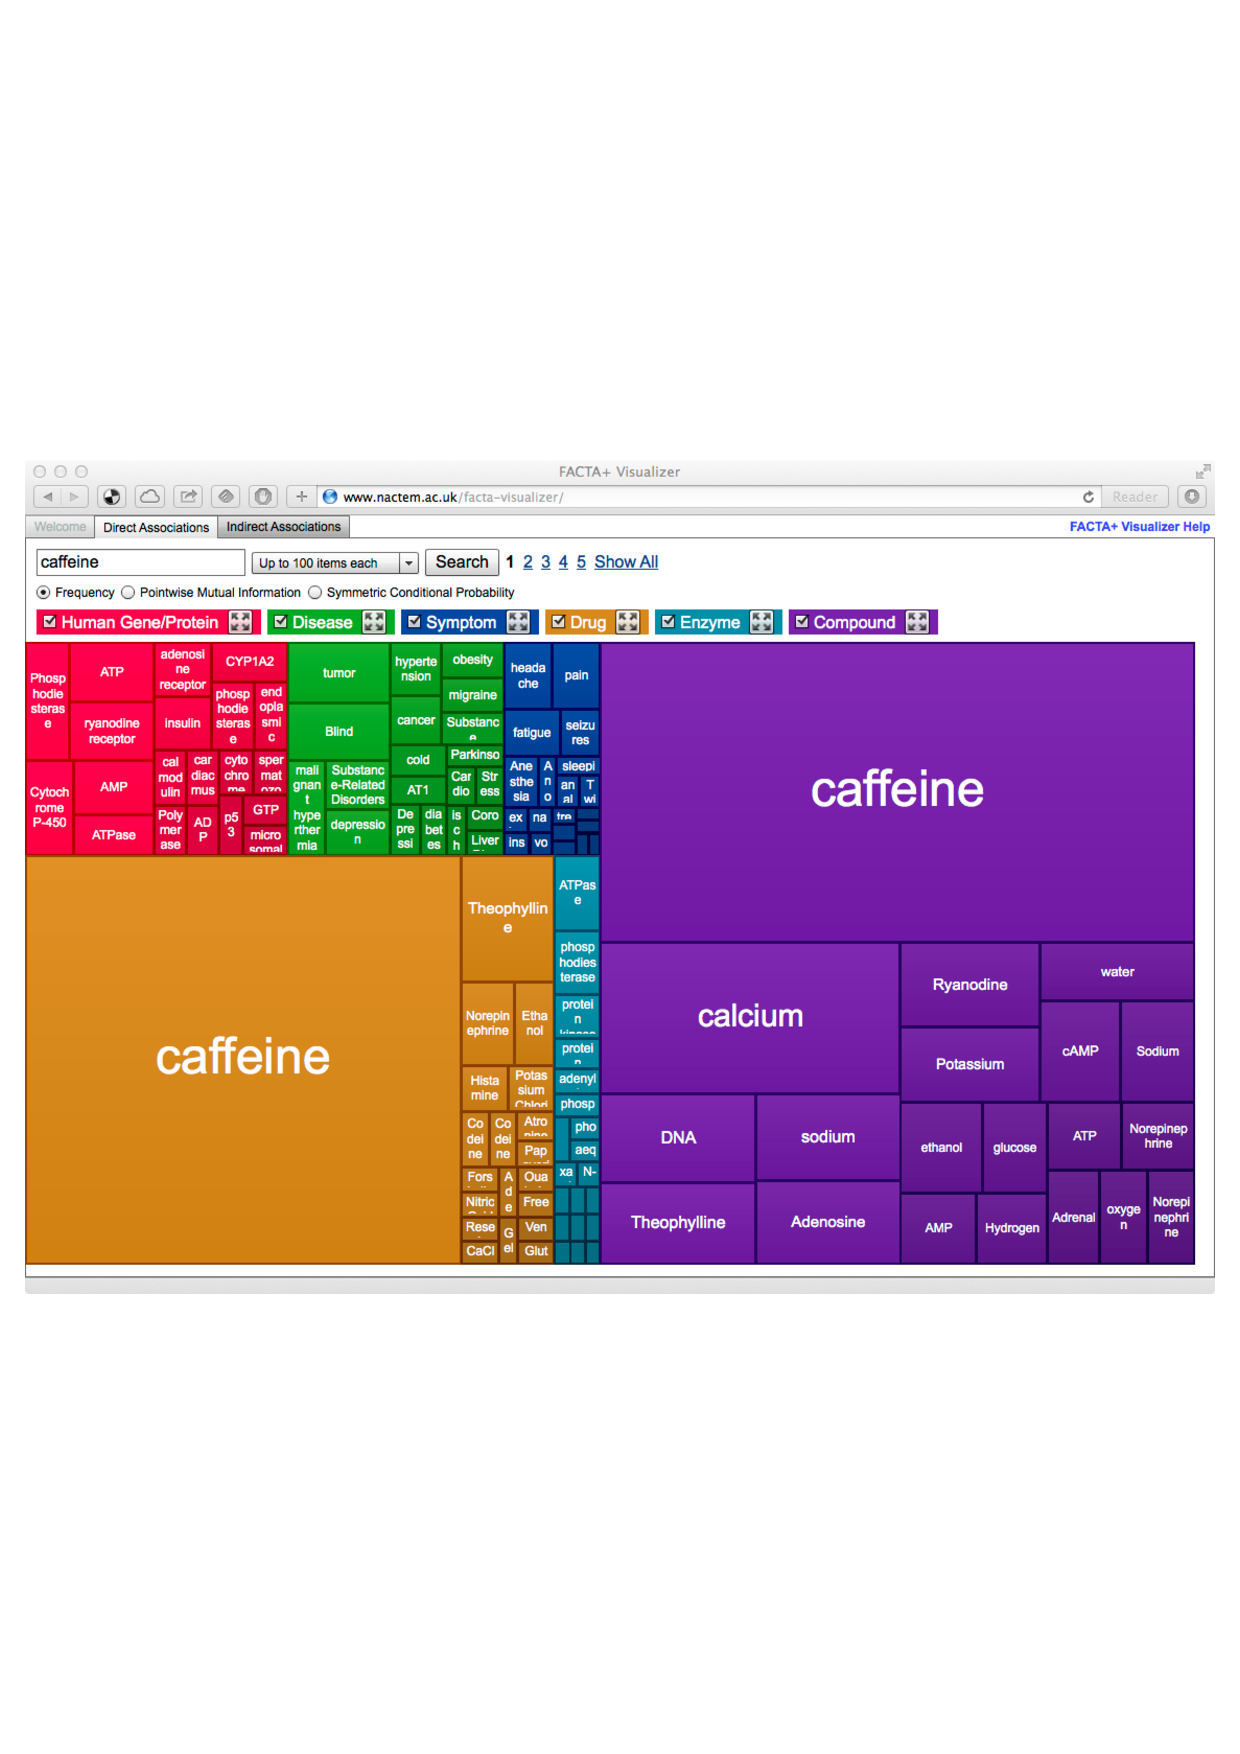
\includegraphics[scale=0.6]{figures/facta-vis.pdf}
 \caption{FACTA+ graphical visualisation showing concepts associated to ``caffeine'' }
\label{fig:facta-vis}
\end{center}
\end{figure}


\EM{More examples of applications/systems for text mining in biomedicine}


\section{Tools for Text Mining in Biomedicine}
\label{sec:tools-tm}

\subsection{Entity Detection}

\emph{Entity detection} -- often called named \emph{entity recognition} (NER) in other areas of NLP -- is the process of detecting mentions of entities in text.
Generic enitity detection tools are not well-suited for biomedical text because of highly specialized language use (jargon). 
For example, many terms have a particular meaning or do not occur at all outside of biomedical texts.
In biomedicine, it is usually quite clear what the entities of interest are, for example, genes, proteins, cells, drugs, organisms, etc.
However, detecting entities is a non-trivial task due to a number of complications.

First, there is variation in spelling and naming of entity names.
For example, a gene name may be spelled as \emph{BRCA 2},\emph{ BRCA-2},\emph{Brca2} or \emph{Brca-2} \citep{Krallinger2010Analysis}.
The use of acronyms or abbreviations instead of full names is common. 
Typos are not uncommon.
All this variation in form means that it usually does not suffice to lookup a string in a given dictionary of named entities.

Second, there is ambiguity: a term may mean different things depending on the context.
This is a common problem in NLP.
For instance, the word \emph{bat} may refer to flying animal or to a hitting instrument, depending on the context of use.
Automatically determining the right sense of a word is called \emph{word sense disambiguation}.
In biomedicine, this is often referred to as \emph{entity normalization}, where each entity mention is linked to a unique indentifier in a database, controlled vocabulary or ontology, so its meaning becomes unambiguous. 
 
Third, as science progresses in certain domain, so does the sublanguage to describe it, and consequently new terms are added all the time.
This means that systems for entity detection must be updated all the time. 
In addition, terms may gradually change meaning over time, a phenomenon known as \emph{semantic drift}.

\subsection{Relation Extraction}   

, relation extarRelation extraction aims at automatic extraction of relations between entities from text.
There is basically two approaches to relation extraction: co-occurence-based approaches and NLP-based approaches.

Co-occurence-based relation extraction follows a statistical approach. It infers that there is a relation between two entities whenever they tend to occur together frequently. 
The scope of co-occurrence can be within a fixed-sized window, a sentence, a paragraph or even a whole document. 
Different measures have been proposed to compute the association strenght between entities, but essentially all of these measure if two entities occur together more often than is to be expected by chance. 
Co-occurence-based extraction does not require any advanced NLP, so it fairly robust against e.g. very complex or ill-formed input. It tends to give high recall at the cost of low precision. 
That is, it tends to identify most of the true relations but also suggests many false relations. 
In addition, relations are non-directional, which makes the approach suitable for only certain types of relation (e.g. correlation) but unsuitable for others (e.g. causality).
NLP-based relation extraction targets binary relations such as ``protein X activates gene Y'', ``drug X treats disease Y'' or ``gene X is associated with disease Y''.
It is usually assumed that entities are already detected prior to relation extraction and that the set of targeted relations is very limited.
Still, relation extraction is a hard task because of the variation, ambiguity and vagueness in language use.
There are so many different ways to express essentially the same relation in language, that listing all of them is practically impossible: there will always be new ways to say the same thing.
Hence straight forward lookup or template matching on the word level is bound to fail.
Most systems first perform a linguistic analysis step, resulting in a more abstract representation ranging from a normalized surface string to hihh-level syntactic or semantic graph structures. 
Relations are then extracted by manually written pattern matching rules operating on these abstract representations.
Alternatively, and more popular nowadays, extraction is performed in a data-driven fashion, where supervised machine learning algorithms learn to recognize relations from training examples.
This requires an annotated corpus of text material in which relations are labeled by human annotators.
NLP-based extraction systems are more brittle, because they depend very much on the quality of the NLP tools such as part-of-speech taggers and syntactic parsers.
They tends to give high precision but low recall.
They are also more expensive to build, because of manual labour involved in writing pattern matching rules or annotating training corpora.
However, extracted relations can be directional, which makes them potentially more useful for many applications. 

Hybrid systems combine different approaches, sometimes both co-occurence-based and NLP-based, to obtain better performance.
Another recent trend is to perform entitity recognition and relation extraction simultaneously in a single unified system.
This potentially avoids error propagation in cases where failure to detect the correct entities prevents extraction of the correct relation.
  
\subsection{Event Extraction}

Event extraction may be regarded as a generalization of relation extraction.
Where relation extraction is limited to binary relations between two entities, events can involve multiple entities.
These are labeled according to the role they play in the event, often called \emph{thematic roles}.
Moreover, one event can play the role in another event, giving rise to recursive structures.
Figure~\ref{fig:event-example} shows an example of an event from the BioNLP event extraction task.
It has an event called \emph{Phosphorylation} that applies to the protein STAT3, which therefore plays the role of \emph{Theme} in this event.
This \emph{Phosphorylation} event in turn plays the role of \emph{Theme} in another event called \emph{Regulation}, which also involves the protein Vav in the role of \emph{Cause}.
A third event takes the same \emph{Theme} role (\emph{Phosphorylation}) but a different \emph{Cause} (Rac-1).

\begin{figure}
\begin{center}
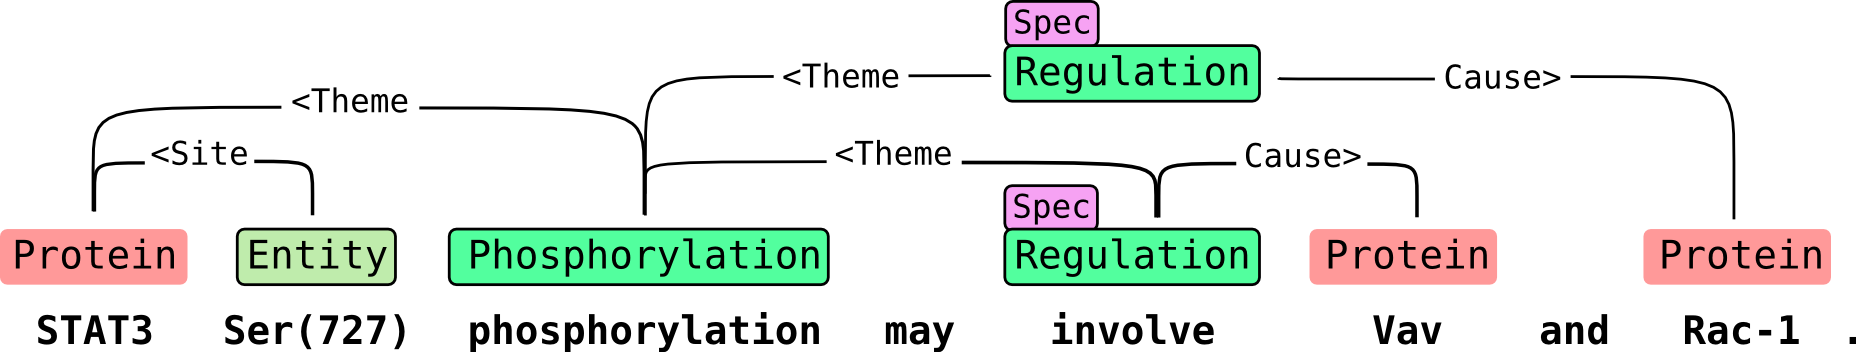
\includegraphics[scale=0.65]{figures/event-example.png}
 \caption{Example of an event from the BioNLP event extraction task \citep{Bjorne2011EXTRACTING}}
\label{fig:event-example}
\end{center}
\end{figure}

Event extraction are almost exclusively NLP-based and usually involve syntactic parsing.
It is closely related to the task of \emph{semantic role labelling} (SRL) which aims to label predicates and their semantic roles according to some general linguistic theory about semantic frames. 
Approaches can be knowledge-based (hand-written rules), data-driven (supervised machine learning) or hybrid.
Probabably the most succesful event extraction system for biomedicine acording to recent system evaluations is the Turku Event Extraction Systeem (TEES), which is a machine learning system employing support vector machines in combination with separate systems for entitity detection and syntactic parsing \citep{Bjorne2011EXTRACTING}. 

Recently particular aspects of events have extracted attention, for example, negation and speculation. Negation detection systems try to detect if an event is in the scope of a of negation -- e.g. \emph{not}, \emph{neither} or \emph{lack of evidence for}. 
Evidently, knowing that a fact is negated is crucial in any text mining application.
Likewise, detection of speculation, modality, uncertainty or hedging provides important information.
For example, an event may be qualified as \emph{possible}, \emph{unlikely} or \emph{not always}.
The two regulation events in Figure~\ref{fig:event-example} are marked as \emph{Spec} (speculative) because of the modal verb \emph{may}, which signals a certain amount of uncertainty.

\subsection{Evaluation}

Comparing different approaches proposed to entity detection, relation extraction, event extraction and similar tasks in information extration and text mining is not easy, because results reported in the literature on different text material, or using different evaluation methods and measures, can not be compared with each other.
However, without proper empirical evaluation, it is essentialy impossible to judge if any progress is made.
Several evaluation initiatives in biomedical NLP and text mining have addressed this issue, including the BioCreative and BioNLP shared tasks.
These follow the established practice in NLP and machine learning of providing a standard evaluation framework for a particular task consisting of labeled development data, blind test data and proper evaluation measures.   
Participants build systems for performing the task -- e.g. entity detection -- on the basis of the labeled development data.
They then apply their systems to label the the blind test data.
The shared task organisers compare the system predictions to the true answers (gold standard) according to some evaluation measures, which allows the different systems to be ranked according to their performance on the task.
Systematic comparison of the performance of different methods, in combination with detailed error analysis, defines the state-of-the-art and suggests ways for further improvement.

Although this methodology has been instrumental in progressing the field, it is not without its disadvantages.
For instance, systems are known to become overfitted on the type of text used in the evaluation.
Applying the same system to text from a different domain may lead to dramatic drops in performance. 

\section{Machine Reading and Open Information Extraction}

There are two other areas which are closely related to text mining, both involving NLP.
The idea of \emph{machine reading} is essentially to enable computers to read text in electronic format, understand its meaning and extract knowledge from it in the same way as humans do \citep{Mitchell2005Reading}.
Given the enormous amount of computer-readable text available on the internet and from scanned books, a functional machine reading system would allow computational agents to acquire knowledge on an unprecedented scale.
\emph{Open information extraction} also aims for knowledge base population through informatin extraction from text \citet{banko2007open,Etzioni2011Search}.
In contrast to traditional information extraction, where there is a fixed set predetermined relations, in open IE the set of relations is open, that is, any relation encoded in text is targeted.  
Examples include the TextRunner open IE system and its succesors \citep{yates2007textrunner}, the DeepDive system \citep{niu2012deepdive}, CMU's Never Ending Language Learner (NELL) \citep{carlson-aaai} that learns to extract facts from the webpages,  MPI's YAGO system that learns fact from Wikipedia and combines them with WordNet \citep{YAGO} and IBM's Watson system that played Jeopardy \citep{fan2012automatic}.

\todo[inline]{inference and reasoning, relation to GOFAI}


%%% Local Variables: 
%%% mode: latex
%%% TeX-master: "ocwp1-d1"
%%% End: 

 